\documentclass{beamer}
\usepackage[T1]{fontenc}
\usepackage[utf8]{inputenc}

\usetheme{Madrid}
\usecolortheme{default}
\usepackage{amsmath,amssymb,amsfonts,amsthm}
\usepackage{txfonts}
\usepackage{tkz-euclide}
\usepackage{listings}
\usepackage{adjustbox}
\usepackage{array}
\usepackage{tabularx}
\usepackage{gvv}
\usepackage{lmodern}
\usepackage{gensymb}
\usepackage{circuitikz}
\usepackage{tikz}
\usepackage{graphicx}
\usepackage{capt-of}

\setbeamertemplate{page number in head/foot}[totalframenumber]

\usepackage{tcolorbox}
\tcbuselibrary{minted,breakable,xparse,skins}

\definecolor{bg}{gray}{0.95}
\DeclareTCBListing{mintedbox}{O{}m!O{}}{%
  breakable=true,
  listing engine=minted,
  listing only,
  minted language=#2,
  minted style=default,
  minted options={%
    linenos,
    gobble=0,
    breaklines=true,
    breakafter=,,
    fontsize=\small,
    numbersep=8pt,
    #1},
  boxsep=0pt,
  left skip=0pt,
  right skip=0pt,
  left=25pt,
  right=0pt,
  top=3pt,
  bottom=3pt,
  arc=5pt,
  leftrule=0pt,
  rightrule=0pt,
  bottomrule=2pt,
  toprule=2pt,
  colback=bg,
  colframe=orange!70,
  enhanced,
  overlay={%
    \begin{tcbclipinterior}
    \fill[orange!20!white] (frame.south west) rectangle ([xshift=20pt]frame.north west);
    \end{tcbclipinterior}},
  #3,
}
\lstset{
    language=C,
    basicstyle=\ttfamily\small,
    keywordstyle=\color{blue},
    stringstyle=\color{orange},
    commentstyle=\color{green!60!black},
    numbers=left,
    numberstyle=\tiny\color{gray},
    breaklines=true,
    showstringspaces=false,
}

\title{2.3.13}
\subtitle{Vector Geometry}
\author{EE25BTECH11010 - Arsh Dhoke}
\date{}

\begin{document}

\begin{frame}
\titlepage
\end{frame}

\begin{frame}{Question}
Find the angle which the line $\frac{x}{1}=\frac{y}{-1}=\frac{z}{2}$ makes with the positive direction of the Y axis.
\end{frame}

\begin{frame}{Angle Between Line and Y-axis}
The line can be represented as 
$
k \myvec{1\\-1\\2}
$

Hence its direction vector is

\begin{align}
\vec{v} &= \myvec{1\\-1\\2} \\
\vec{e_2} &= \myvec{0\\1\\0} \\
\vec{v}^T\vec{e_2} &= 
\myvec{1 & -1 & 2}\myvec{0\\1\\0}=-1 
\end{align}
\end{frame}

\begin{frame}{Calculation}
\begin{align}
\|\vec{v}\| &= 
\sqrt{\vec{v}^T\vec{v}}
=\sqrt{\myvec{1 & -1 & 2}\myvec{1\\-1\\2}}=\sqrt{6} \\
\|\vec{e_2}\| &=1 \\
\cos\theta &= 
\frac{\vec{v}^T\vec{e_2}}{\|\vec{v}\|\|\vec{e_2}\|}
=\frac{-1}{\sqrt{6}} \\
\theta &= \cos^{-1}\!\brak{-\frac{1}{\sqrt{6}}}
\end{align}
$
\boxed{\theta=\cos^{-1}\!\brak{-\frac{1}{\sqrt{6}}}\;\approx\;114.09\degree}
$
\end{frame}

\begin{frame}{Plot}
\centering
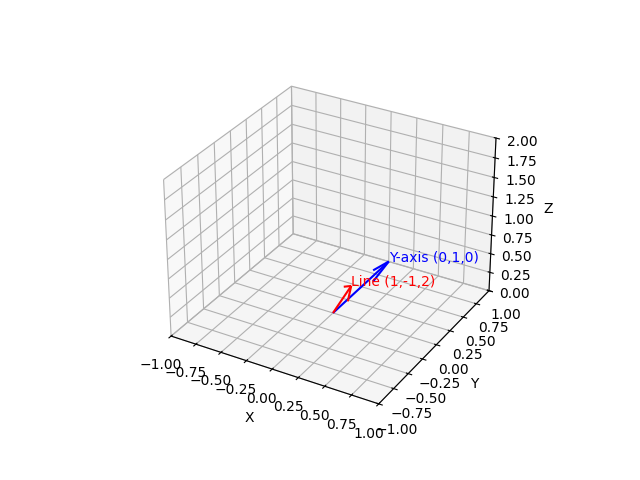
\includegraphics[height=0.6\textheight, keepaspectratio]{figs/q3.png}
\captionof{figure}{Graph}
\end{frame}

\begin{frame}[fragile]
    \frametitle{C Code}
\begin{lstlisting}
#include <stdio.h>
#include <math.h>

double angleWithYAxis(double vx, double vy, double vz) {
    double e2y = 1.0;
    double dot = vy * e2y;
    double magv = sqrt(vx*vx + vy*vy + vz*vz);
    double mage2 = 1.0;
    double cosTheta = dot / (magv * mage2);
    double thetaRad = acos(cosTheta);
    double thetaDeg = thetaRad * 180.0 / M_PI;
    return thetaDeg;
}
int main() {
    double vx = 1, vy = -1, vz = 2;
    double theta = angleWithYAxis(vx, vy, vz);
    printf("Angle with positive Y-axis = %.2f degrees\n", theta);
    return 0;
}
\end{lstlisting}
\end{frame}

\begin{frame}[fragile]
    \frametitle{Python Code}
\begin{lstlisting}
import numpy as np
import matplotlib.pyplot as plt
from mpl_toolkits.mplot3d import Axes3D

# Vectors
v = np.array([1, -1, 2])
e2 = np.array([0, 1, 0])

# Normalize for plotting
v_unit = v / np.linalg.norm(v)
e2_unit = e2 / np.linalg.norm(e2)

fig = plt.figure()
ax = fig.add_subplot(111, projection='3d')

origin = np.array([0, 0, 0])

# Plot vectors
\end{lstlisting}
\end{frame}

\begin{frame}[fragile]
    \frametitle{Python Code}
\begin{lstlisting}
ax.quiver(*origin, *v_unit, color='r')
ax.quiver(*origin, *e2_unit, color='b')

# Add labels next to the tips
ax.text(*v_unit, "Line (1,-1,2)", color='r', fontsize=10)
ax.text(*e2_unit, "Y-axis (0,1,0)", color='b', fontsize=10)

# Axes labels and limits
ax.set_xlabel('X')
ax.set_ylabel('Y')
ax.set_zlabel('Z')
ax.set_xlim([-1, 1])
ax.set_ylim([-1, 1])
ax.set_zlim([0, 2])
ax.grid(True)

plt.savefig("/home/arsh-dhoke/ee1030-2025/ee25btech11010/matgeo/2.3.13/figs/q3.png")
plt.show()

\end{lstlisting}
\end{frame}

\begin{frame}[fragile]
    \frametitle{Python+ C Code}
\begin{lstlisting}
import numpy as np
import matplotlib.pyplot as plt
from ctypes import CDLL, c_double

# Load the shared library
lib = CDLL("./code.so")  # use your code.so file

# Define argument and return types
lib.angleWithYAxis.argtypes = [c_double, c_double, c_double]
lib.angleWithYAxis.restype = c_double

# Vector
vx, vy, vz = 1.0, -1.0, 2.0

# Call C function
theta_deg = lib.angleWithYAxis(vx, vy, vz)
print(f"Angle with positive Y-axis = {theta_deg:.2f} degrees")

\end{lstlisting}
\end{frame}

\begin{frame}[fragile]
    \frametitle{Python+ C Code}
\begin{lstlisting}
# 3D plotting
v = np.array([vx, vy, vz])
e2 = np.array([0, 1, 0])  # Y-axis unit vector

# Normalize for plotting
v_unit = v / np.linalg.norm(v)
e2_unit = e2 / np.linalg.norm(e2)

fig = plt.figure()
ax = fig.add_subplot(111, projection='3d')
origin = np.array([0, 0, 0])

# Plot vectors
ax.quiver(*origin, *v_unit, color='r', length=1)
ax.quiver(*origin, *e2_unit, color='b', length=1)

# Labels
\end{lstlisting}
\end{frame}

\begin{frame}[fragile]
    \frametitle{Python+ C Code}
\begin{lstlisting}
ax.text(*(v_unit + 0.1), f"Line {tuple(v)}", color='r', fontsize=10)
ax.text(*(e2_unit + 0.1), f"Y-axis {tuple(e2)}", color='b', fontsize=10)
ax.text(0.2, 0.2, 0.2, f"Angle with Y-axis: {theta_deg:.2f}°", color='k', fontsize=12)

# Axes
ax.set_xlabel('X')
ax.set_ylabel('Y')
ax.set_zlabel('Z')
ax.set_xlim([-1, 1])
ax.set_ylim([-1, 1])
ax.set_zlim([0, 2])
ax.grid(True)

plt.savefig("/home/arsh-dhoke/ee1030-2025/ee25btech11010/matgeo/2.3.13/figs/q3.png")
plt.show()

\end{lstlisting}
\end{frame}

\end{document}